\section{Statistical Analysis}
\label{sec:analysis:method}



Having carried out the event selection as described in section~\ref{sec:analysis:selection}, the estimation of the W branching fraction is carried out using two different approaches.  Before describing the two approaches, it will be useful to describe the formalism that is common to both.


%%%%%%%%%%%%%%%%%%%%%%%%%%%%%%%%%%%%%%%%
% 1. Determination of Signal Acceptance
%%%%%%%%%%%%%%%%%%%%%%%%%%%%%%%%%%%%%%%%
\subsection{Determination of Signal Efficiency}

For single W decay, also taking into account the $\tau$ decay, we write the branching 
ratio in the form of a vector

\begin{equation}
    \vec{B} = 
    \begin{bmatrix}
        B_e & B_\mu & B_{\tau_e} & B_{\tau_\mu} &  B_{\tau_h} & B_h
	\end{bmatrix} 
\end{equation}

For WW decay, there are 21 possible final states. We can denote the branching
ratio as a 6-by-6 symmetric matrix with 21 independent terms. Mathematically, 
this branching ratio matrix \textit{B} equals to the outer product of vector
$\vec{B}$:

\begin{equation}
	B = \vec{B}^T \vec{B} =
    \begin{bmatrix}
        B_e B_e             & B_e B_\mu         & B_e B_{\tau_e}            & B_e B_{\tau_\mu}          & B_e B_{\tau_h}            & B_e B_h           \\
        B_\mu B_e           & B_\mu B_\mu       & B_\mu B_{\tau_e}          & B_\mu B_{\tau_\mu}        & B_\mu B_{\tau_h}          & B_\mu B_h         \\
        B_{\tau_e} B_e      & B_{\tau_e} B_\mu  & B_{\tau_e} B_{\tau_e}     & B_{\tau_e} B_{\tau_\mu}   & B_{\tau_e} B_{\tau_h}     & B_{\tau_e} B_h    \\
        B_{\tau_\mu} B_e    & B_{\tau_\mu}B_\mu & B_{\tau_\mu} B_{\tau_e}   & B_{\tau_\mu} B_{\tau_\mu} & B_{\tau_\mu} B_{\tau_h}   & B_{\tau_\mu} B_h  \\
        B_{\tau_h} B_e      & B_{\tau_h} B_\mu  & B_{\tau_h} B_{\tau_e}     & B_{\tau_h}  B_{\tau_\mu}  & B_{\tau_h} B_{\tau_h}     & B_{\tau_h} B_h    \\
        B_h B_e             & B_h B_\mu         & B_h B_{\tau_e}            & B_h B_{\tau_\mu}          & B_h  B_{\tau_h}           & B_h  B_h 
	\end{bmatrix}
	\label{eq:br_matrix}
\end{equation}


Similarly, signal efficiency has 21 independent terms, corresponding to 21
WW decay channels. In each channel, we defining $E$ matrix to manage these terms.

\begin{equation}
	E = 
	\begin{bmatrix}
    E_{ee}          & E_{e\mu}          & E_{e\tau_e}       & E_{e\tau_\mu}        & E_{e\tau_h}        & E_{eh}        \\
    E_{\mu e}       & E_{\mu \mu}       & E_{\mu \tau_e}    & E_{\mu \tau_\mu}     & E_{\mu \tau_h}     & E_{\mu h}     \\
    E_{\tau_e e}    & E_{\tau_e \mu}    & E_{\tau_e \tau_e} & E_{\tau_e \tau_\mu}  & E_{\tau_e \tau_h}  & E_{\tau_e h}  \\
    E_{\tau_\mu e}  & E_{\tau_\mu\mu}   & E_{\tau_\mu\tau_e}& E_{\tau_\mu\tau_\mu} & E_{\tau_\mu\tau_h} & E_{\tau_\mu h}\\
    E_{\tau_h e}    & E_{\tau_h \mu}    & E_{\tau_h \tau_e} & E_{\tau_h \tau_\mu}  & E_{\tau_h \tau_h } & E_{\tau_h h}  \\
    E_{he}          & E_{h\mu}          & E_{h\tau_e}       & E_{h\tau_\mu}        & E_{h\tau_h}        & E_{hh} 
	\end{bmatrix}
    \label{eq:eff_matrix}
\end{equation}


In counting analysis, the signal efficiency is therefore slightly differ 
from shape analysis because of slightly higher pT threshold in $\mu\tau$, $\mu4j$ channel
and tighter tau working point. In 8 channels in 1b and 2b cases, the signal efficiency 
is determined from $t\bar{t}$ and {tW} MC events, with result being shown in Figure 
\ref{efficencyMatrix} and Table \ref{efficencyTableMuon}, \ref{efficencyTableElectron}.
In addition, the percentage portion of each of 21 WW decay final states is 
shown in Table \ref{selectionSignals}.

With the E and B matrix, the prediction of yield in a channel can be expressed as

\begin{equation}
    N = \sigma_{sg}L\times \textbf{E} \cdot \textbf{B} + \sum N_{bg}
    \label{prediction}
\end{equation}


\begin{figure}[ht]
    \centering
    channels with $\mu$-trigger-1b \\
    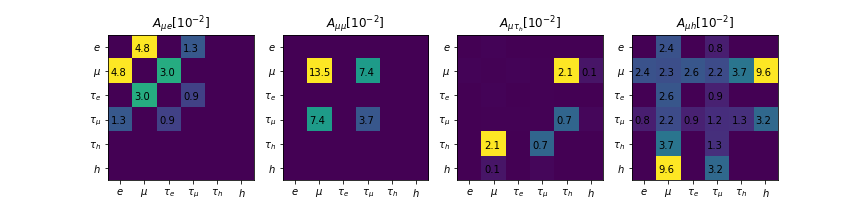
\includegraphics[width=15cm]{chapters/Analysis/sectionStatisticalAnalysis/figures/acc_mu1b.png}
    
    channels with $\mu$-trigger-2b \\
    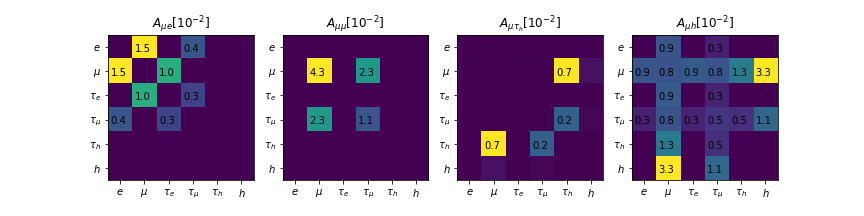
\includegraphics[width=15cm]{chapters/Analysis/sectionStatisticalAnalysis/figures/acc_mu2b.png}
    
    channels with $e$-trigger-1b \\
    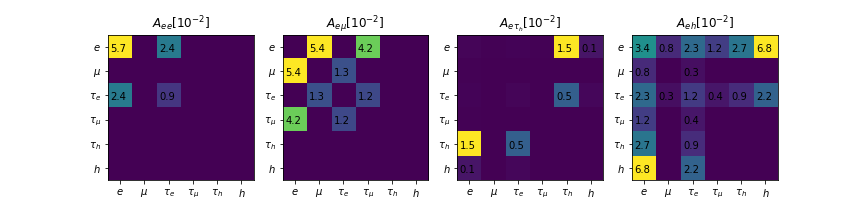
\includegraphics[width=15cm]{chapters/Analysis/sectionStatisticalAnalysis/figures/acc_e1b.png}
    
    channels with $e$-trigger-2b \\
    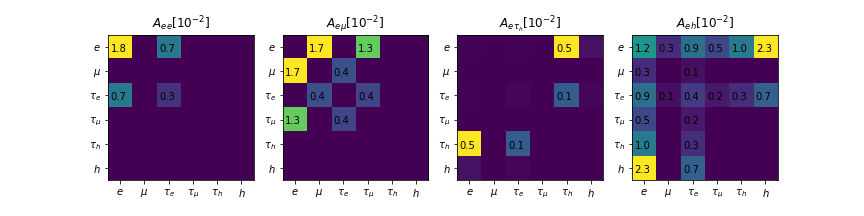
\includegraphics[width=15cm]{chapters/Analysis/sectionStatisticalAnalysis/figures/acc_e2b.png}
    
    %--------------------------
    \caption{ Efficiency matrices \textbf{E} in trigger and b-tag categories. }
    \label{efficencyMatrix}
\end{figure}

\begin{sidewaystable}[p]
    \centering
    \setlength{\tabcolsep}{0.4em}
    \renewcommand{\arraystretch}{1.5}
    \caption{Efficiency of $t\bar{t}$+$tW$ events, breakdown by 21 WW decay.  Values are in percent.}
    
    \resizebox{\textwidth}{!}{
    \begin{tabular}{|l|cc|cc|cc|cc|cc|cc|cc|cc|}
    
    
    \hline
    channel & \multicolumn{2}{|c|}{$\mu e$} & \multicolumn{2}{c|}{$\mu\mu$} & \multicolumn{2}{|c|}{$\mu \tau$} & \multicolumn{2}{|c|}{$\mu$+jets} & \multicolumn{2}{|c|}{$ee$} & \multicolumn{2}{|c|}{$e\mu$} & \multicolumn{2}{|c|}{$e \tau$} & \multicolumn{2}{|c|}{$e+jets$} \\
    \hline
    $\rm n_{b tag}$ & $n_b=1$ & $n_b\geq2$ & $n_b=1$ & $n_b\geq2$ & $n_b=1$ & $n_b\geq2$ & $n_b=1$ & $n_b\geq2$ & $n_b=1$ & $n_b\geq2$ & $n_b=1$ & $n_b\geq2$ & $n_b=1$ & $n_b\geq2$ & $n_b=1$ & $n_b\geq2$ \\ 
    \hline
    
    $tt/tW \to ee$                     &    --    &    --    &    --    &    --    &    --    &    --    &    --    &    --    &  5.71(1) &  3.19(1) &    --    &    --    &    --    &    --    &  3.17(1) &  2.14(1) \\ 
    $tt/tW \to \mu\mu$                 &    --    &    --    & 14.14(2) &  8.02(1) &    --    &    --    &  1.80(1) &  1.21(0) &    --    &    --    &    --    &    --    &    --    &    --    &    --    &    --    \\ 
    $tt/tW \to e\mu$                   &  4.69(1) &  2.66(0) &    --    &    --    &    --    &    --    &  2.35(0) &  1.60(0) &    --    &    --    &  5.76(1) &  3.24(1) &    --    &    --    &  0.71(0) &  0.48(0) \\ 
    $tt/tW \to \tau_{e}\tau_{e}$       &    --    &    --    &    --    &    --    &    --    &    --    &    --    &    --    &  0.74(2) &  0.44(2) &    --    &    --    &    --    &    --    &  1.18(4) &  0.81(2) \\ 
    $tt/tW \to \tau_{\mu}\tau_{\mu}$   &    --    &    --    &  3.88(5) &  2.11(4) &    --    &    --    &  1.13(3) &  0.77(2) &    --    &    --    &    --    &    --    &    --    &    --    &    --    &    --    \\ 
    $tt/tW \to \tau_{e}\tau_{\mu}$     &  0.78(2) &  0.45(1) &    --    &    --    &    --    &    --    &  0.92(2) &  0.62(1) &    --    &    --    &  1.24(2) &  0.70(2) &    --    &    --    &  0.40(1) &  0.27(1) \\ 
    $tt/tW \to \tau_{e}\tau_{h}$       &    --    &    --    &    --    &    --    &    --    &    --    &    --    &    --    &    --    &    --    &    --    &    --    &  0.48(1) &  0.26(0) &  0.84(1) &  0.61(1) \\ 
    $tt/tW \to \tau_{\mu}\tau_{h}$     &    --    &    --    &    --    &    --    &  0.74(1) &  0.40(1) &  1.28(1) &  0.92(1) &    --    &    --    &    --    &    --    &    --    &    --    &    --    &    --    \\ 
    $tt/tW \to \tau_{h}\tau_{h}$       &    --    &    --    &    --    &    --    &    --    &    --    &    --    &    --    &    --    &    --    &    --    &    --    &    --    &    --    &    --    &    --    \\ 
    $tt/tW \to e\tau_{e}$              &    --    &    --    &    --    &    --    &    --    &    --    &    --    &    --    &  2.14(1) &  1.18(1) &    --    &    --    &    --    &    --    &  2.29(1) &  1.62(1) \\ 
    $tt/tW \to e\tau_{\mu}$            &  1.28(1) &  0.69(1) &    --    &    --    &    --    &    --    &  0.80(1) &  0.54(0) &    --    &    --    &  4.49(2) &  2.47(1) &    --    &    --    &  1.18(1) &  0.86(1) \\ 
    $tt/tW \to e\tau_{h}$              &    --    &    --    &    --    &    --    &    --    &    --    &    --    &    --    &    --    &    --    &    --    &    --    &  1.59(1) &  0.88(0) &  2.61(1) &  1.90(0) \\ 
    $tt/tW \to \mu\tau_{e}$            &  2.54(1) &  1.43(1) &    --    &    --    &    --    &    --    &  2.61(1) &  1.86(1) &    --    &    --    &  1.42(1) &  0.78(1) &    --    &    --    &  0.23(0) &  0.16(0) \\ 
    $tt/tW \to \mu\tau_{\mu}$          &    --    &    --    &  7.76(2) &  4.37(2) &    --    &    --    &  1.88(1) &  1.35(1) &    --    &    --    &    --    &    --    &    --    &    --    &    --    &    --    \\ 
    $tt/tW \to \mu\tau_{h}$            &    --    &    --    &    --    &    --    &  2.27(1) &  1.27(0) &  3.70(1) &  2.70(1) &    --    &    --    &    --    &    --    &    --    &    --    &    --    &    --    \\ 
    $tt/tW \to eh$                     &    --    &    --    &    --    &    --    &    --    &    --    &    --    &    --    &    --    &    --    &    --    &    --    &  0.10(0) &    --    &  6.83(0) &  4.64(0) \\ 
    $tt/tW \to \mu h$                  &    --    &    --    &    --    &    --    &  0.15(0) &    --    &  9.71(1) &  6.61(0) &    --    &    --    &    --    &    --    &    --    &    --    &    --    &    --    \\ 
    $tt/tW \to \tau_{e}h$              &    --    &    --    &    --    &    --    &    --    &    --    &    --    &    --    &    --    &    --    &    --    &    --    &    --    &    --    &  2.17(1) &  1.44(0) \\ 
    $tt/tW \to \tau_{\mu}h$            &    --    &    --    &    --    &    --    &    --    &    --    &  3.30(1) &  2.19(1) &    --    &    --    &    --    &    --    &    --    &    --    &    --    &    --    \\ 
    $tt/tW \to \tau_{h}h$              &    --    &    --    &    --    &    --    &    --    &    --    &    --    &    --    &    --    &    --    &    --    &    --    &    --    &    --    &    --    &    --    \\ 
    $tt/tW \to hh$                     &    --    &    --    &    --    &    --    &    --    &    --    &    --    &    --    &    --    &    --    &    --    &    --    &    --    &    --    &    --    &    --    \\ 

    \hline
    \end{tabular}}
    
    \label{tab:sigacc}
    
\end{sidewaystable}

\FloatBarrier



%%%%%%%%%%%%%%%%%%%%%%%%%%%%%%%%%%%%%%%%
% 2. Extraction of Parameters
%%%%%%%%%%%%%%%%%%%%%%%%%%%%%%%%%%%%%%%%
\subsection{Extraction of Parameters}

In counting analysis, branching fractions are extracted by solving a set of
three quadratic equations, obtained by setting the expected normalized
yields equal to the measured ones. The four measurements are performed independently 
in four mutually exclusive regions based on the number of b tags (1 or more than 2) 
and trigger type (single electron or muon). Then these four measurements are combined based 
on a $\chi^{2}$ minimization to obtain the final result.

The four groups of channels and their yields
are shown in figure~\ref{fig:signalRegion}.
Channels using single-$\mu$ or single-$e$ trigger are

\begin{itemize}
    \item single-$\mu$ trigger : $\mu e$, $\mu\mu$, $\mu\tau$, $\mu h$.
    \item single-$e$ trigger : $ee$, $e\mu$, $e\tau$, $eh$.
\end{itemize}

where $e\mu$ and $\mu e$ are mutually exclusive -- $e\mu$ channel
requires fired e-trigger and \(p^T_e > p^T_\mu\), while $\mu e$ channel
requires fired $\mu$-trigger and \(p^T_e < p^T_\mu\). 

Besides being formally different from the shape analysis, the thresholds
of leptons $p^T$ and working point for the hadronic tau isolation are
slightly different, as optimizations in counting. This results in slightly different signal
acceptances. For the 8 channels under consideration, the signal efficiency determined from
simulated $t\bar{t}$ and tW events are shown in
tables \ref{efficencyTableMuon} and \ref{efficencyTableElectron}. 
The efficiency matrices \textbf{E} of 
included channels in the four categories are shown in Fig \ref{efficencyMatrix}.



The normalized yields, which are inspired by the definition of branching
fraction, is the ratio of one yield over the sum of all yields in the
trigger category:


\begin{itemize}
    \item single-\(\mu\) trigger : 
    \(X_{e} = \frac{n^{\mu e}}{n^{\mu e} + n^{\mu \mu} + n^{\mu \tau} + n^{\mu h}}\), 
    \(X_{\mu} = \frac{n^{\mu \mu}}{n^{\mu e} + n^{\mu \mu} + n^{\mu \tau} + n^{\mu h}}\), 
    \(X_{\tau} = \frac{n^{\mu \tau}}{n^{\mu e} + n^{\mu \mu} + n^{\mu \tau} + n^{\mu h}}\),

    \item single-\(e\) trigger : 
    \(X_{e} = \frac{n^{e e}}{n^{e e} + n^{e \mu} + n^{e \tau} + n^{e h}}\), 
    \(X_{\mu} = \frac{n^{e \mu}}{n^{e e} + n^{e \mu} + n^{e \tau} + n^{e h}}\), 
    \(X_{\tau} = \frac{n^{e \tau}}{n^{e e} + n^{e \mu} + n^{e \tau} + n^{e h}}\),
\end{itemize}

where \(n^f \equiv N^f - \sum_{k\in bg} N^f_k \) is the yield of channel
\(f\) with background subtracted. Based on Eqn \ref{eq:data_model}, the measured normalized yields
\(\{X_{e},X_{\mu},X_{\tau}\}\) should equal to the calculation with
efficiency \textbf{E} and branching fraction \textbf{B}:

\begin{equation} \label{quadEqA}
    \begin{split}
    X_e &= \frac{ E_{ij}^{te}B^{ij} }{E_{ij}^{te}B^{ij} + E_{ij}^{t\mu}B^{ij} + E_{ij}^{t\tau}B^{ij} + E_{ij}^{th}B^{ij}} \\
    X_\mu &= \frac{ E_{ij}^{t\mu}B^{ij} }{E_{ij}^{te}B^{ij} + E_{ij}^{t\mu}B^{ij} + E_{ij}^{t\tau}B^{ij} + E_{ij}^{th}B^{ij}} \\
    X_\tau &= \frac{ E_{ij}^{t\tau}B^{ij} }{E_{ij}^{te}B^{ij} + E_{ij}^{t\mu}B^{ij} + E_{ij}^{t\tau}B^{ij} + E_{ij}^{th}B^{ij}}
    \end{split}
\end{equation}



% where $n^f \equiv N^f - \sum_{k\in bg} n^f_k $ is the yield of channel $f$ 
% with background subtracted and three normalized yields, 
% $\{r_{e},r_{\mu},r_{\tau}\}$, are measured from data with background subtracted. 

% Based on Eqn \ref{prediction}, the measured normalized yields $\{r_{e},r_{\mu},r_{\tau}\}$ 
% should equal to the calculation with efficiency \textbf{E} and branching fraction \textbf{B}:




where \(t\in \{\mu,e\}\) depends on the trigger category. Plugging in
explicit form of \textbf{E} and \textbf{B} matrices in Eqn \ref{eq:br_matrix} and Eqn \ref{eq:eff_matrix}
and unity condition of branching fraction \(\beta_h = 1- \beta_e -
\beta_\mu - \beta_\tau\), Eq \ref{quadEqA} can be written as a set of
three quadratic equations with
\(\{\beta_{e},\beta_{\mu},\beta_{\tau}\}\) as three unknowns.


\begin{equation} \label{quadEqB}
    \footnotesize
	\begin{split}
        Q_e(\beta_e,\beta_\mu,\beta_\tau) &=
        c_{e1} \beta_e^2 + c_{e2} \beta_\mu^2 + c_{e3} \beta_\tau^2 + 
        c_{e4} \beta_e\beta_\mu + c_{e5} \beta_e\beta_\tau + c_{e6} \beta_\mu\beta_\tau +
        c_{e7} \beta_e + c_{e8} \beta_\mu + c_{e9} \beta_\tau + c_{e0} = 0 \\
        %
        Q_\mu(\beta_e,\beta_\mu,\beta_\tau) &= 
        c_{\mu 1} \beta_e^2 + c_{\mu 2} \beta_\mu^2 + c_{\mu 3} \beta_\tau^2 + 
        c_{\mu 4} \beta_e\beta_\mu + c_{\mu 5} \beta_e\beta_\tau + c_{\mu 6} \beta_\mu\beta_\tau +
        c_{\mu 7} \beta_e + c_{\mu 8} \beta_\mu + c_{\mu 9} \beta_\tau + c_{\mu 0} = 0 \\
        %
        Q_\tau(\beta_e,\beta_\mu,\beta_\tau) &= 
        c_{_\tau1} \beta_e^2 + c_{\tau2} \beta_\mu^2 + c_{\tau3} \beta_\tau^2 + 
        c_{\tau4} \beta_e\beta_\mu + c_{\tau5} \beta_e\beta_\tau + c_{\tau6} \beta_\mu\beta_\tau +
        c_{\tau7} \beta_e + c_{\tau8} \beta_\mu + c_{\tau9} \beta_\tau + c_{\tau0} = 0 
    \end{split}
\end{equation}

where coefficients $c_{ei},c_{\mu i},c_{\tau i}$ are fully determined 
by efficiency \textbf{E} and normalized yields $\{X_{e},X_{\mu},X_{\tau}\}$,
as are listed in table~\ref{quadcoeff}.

\begin{table}[ht]
    \centering
   	\setlength{\tabcolsep}{0.4em}
    \renewcommand{\arraystretch}{1.5}
    \small
    
    \begin{tabular}{c|l}

    \hline
    $c_{l0}$ & $\Delta_{hh}$ \\
    \hline
    $c_{l1}$ & $\Delta_{ee}     - 2\Delta_{eh}   + \Delta_{hh}$ \\
    \hline
    $c_{l2}$ & $\Delta_{\mu\mu} - 2\Delta_{\mu h} + \Delta_{hh}$ \\
    \hline
    
    $c_{l3}$ & $   b^\tau_e   b^\tau_e   \Delta_{\tau_e   \tau_e}  
    			 + b^\tau_\mu b^\tau_\mu \Delta_{\tau_\mu \tau_\mu}
                 + b^\tau_h   b^\tau_h   \Delta_{\tau_h   \tau_h}
                 
                 + 2 b^\tau_e   b^\tau_\mu \Delta_{\tau_e   \tau_\mu} 
    		     + 2 b^\tau_e   b^\tau_h   \Delta_{\tau_e   \tau_h}   
    		     + 2 b^\tau_\mu b^\tau_h   \Delta_{\tau_\mu \tau_h} - $ \\
                 
             & $   2 b^\tau_e   \Delta_{e   \tau_h}
                 - 2 b^\tau_\mu \Delta_{\mu \tau_h}
                 - 2 b^\tau_h   \Delta_{h.  \tau_h} 
                 + \Delta_{hh} $ \\

    \hline
    $c_{l4}$ & $2\Delta_{e\mu} - 2\Delta_{eh} -2\Delta_{\mu h} +2\Delta_{hh}$  \\
    \hline
    $c_{l5}$ & $  2b^\tau_e   \Delta_{e \tau_e} 
    			+ 2b^\tau_\mu \Delta_{e \tau_\mu}
                + 2b^\tau_h   \Delta_{e \tau_h}
                - 2b^\tau_e   \Delta_{\tau_e   h} 
    			- 2b^\tau_\mu \Delta_{\tau_\mu h}
                - 2b^\tau_h   \Delta_{\tau_h   h} 
                - 2\Delta_{eh}   + 2 \Delta_{hh} $ \\
        
    \hline            
    $c_{l6}$ & $  2b^\tau_e   \Delta_{\mu \tau_e} 
    			+ 2b^\tau_\mu \Delta_{\mu \tau_\mu}
                + 2b^\tau_h   \Delta_{\mu \tau_h}
                - 2b^\tau_e   \Delta_{\tau_e   h} 
    			- 2b^\tau_\mu \Delta_{\tau_\mu h}
                - 2b^\tau_h   \Delta_{\tau_h   h} 
                - 2\Delta_{\mu h}   + 2 \Delta_{hh} $ \\
    \hline            
    $c_{l7}$ & $ 2\Delta_{eh}      - 2 \Delta_{hh} $ \\
    \hline
    $c_{l8}$ & $ 2\Delta_{\mu h}   - 2 \Delta_{hh}$ \\
    \hline
    $c_{l9}$ & $  2b^\tau_e   \Delta_{\tau_e   h} 
                 + 2b^\tau_\mu \Delta_{\tau_\mu h} 
                 + 2b^\tau_h   \Delta_{\tau_h   h} 
                 - 2 \Delta_{hh}$ \\
    \hline
    \hline
    where  & $ \Delta \equiv E^{tl} - X_l \times ( E^{te} + E^{t\mu} + E^{t\tau} + E^{th} )$ \\
           & $l=e,\mu,\tau$ and $t=e(\mu)$ if using single-$e$ (signle-$\mu$) trigger\\
    \hline
    
	\end{tabular}
    
\caption{ Coefficients of quadratic equations in terms of E and X. In the table, $l=e,\mu,\tau$ and $t=\mu,e$ for single-$\mu$ and single-$e$ trigger respectively.  }
\label{quadcoeff}
    
\end{table}


In the $\{\beta_{e},\beta_{\mu},\beta_{\tau}\}$ parameter space, 
equation~\ref{quadEqB} represents three hyperbolic planes, intersection 
of which is the solution of desired branching fractions, as is shown
in figure~\ref{visualize}.


\begin{figure}[ht]
    \centering
    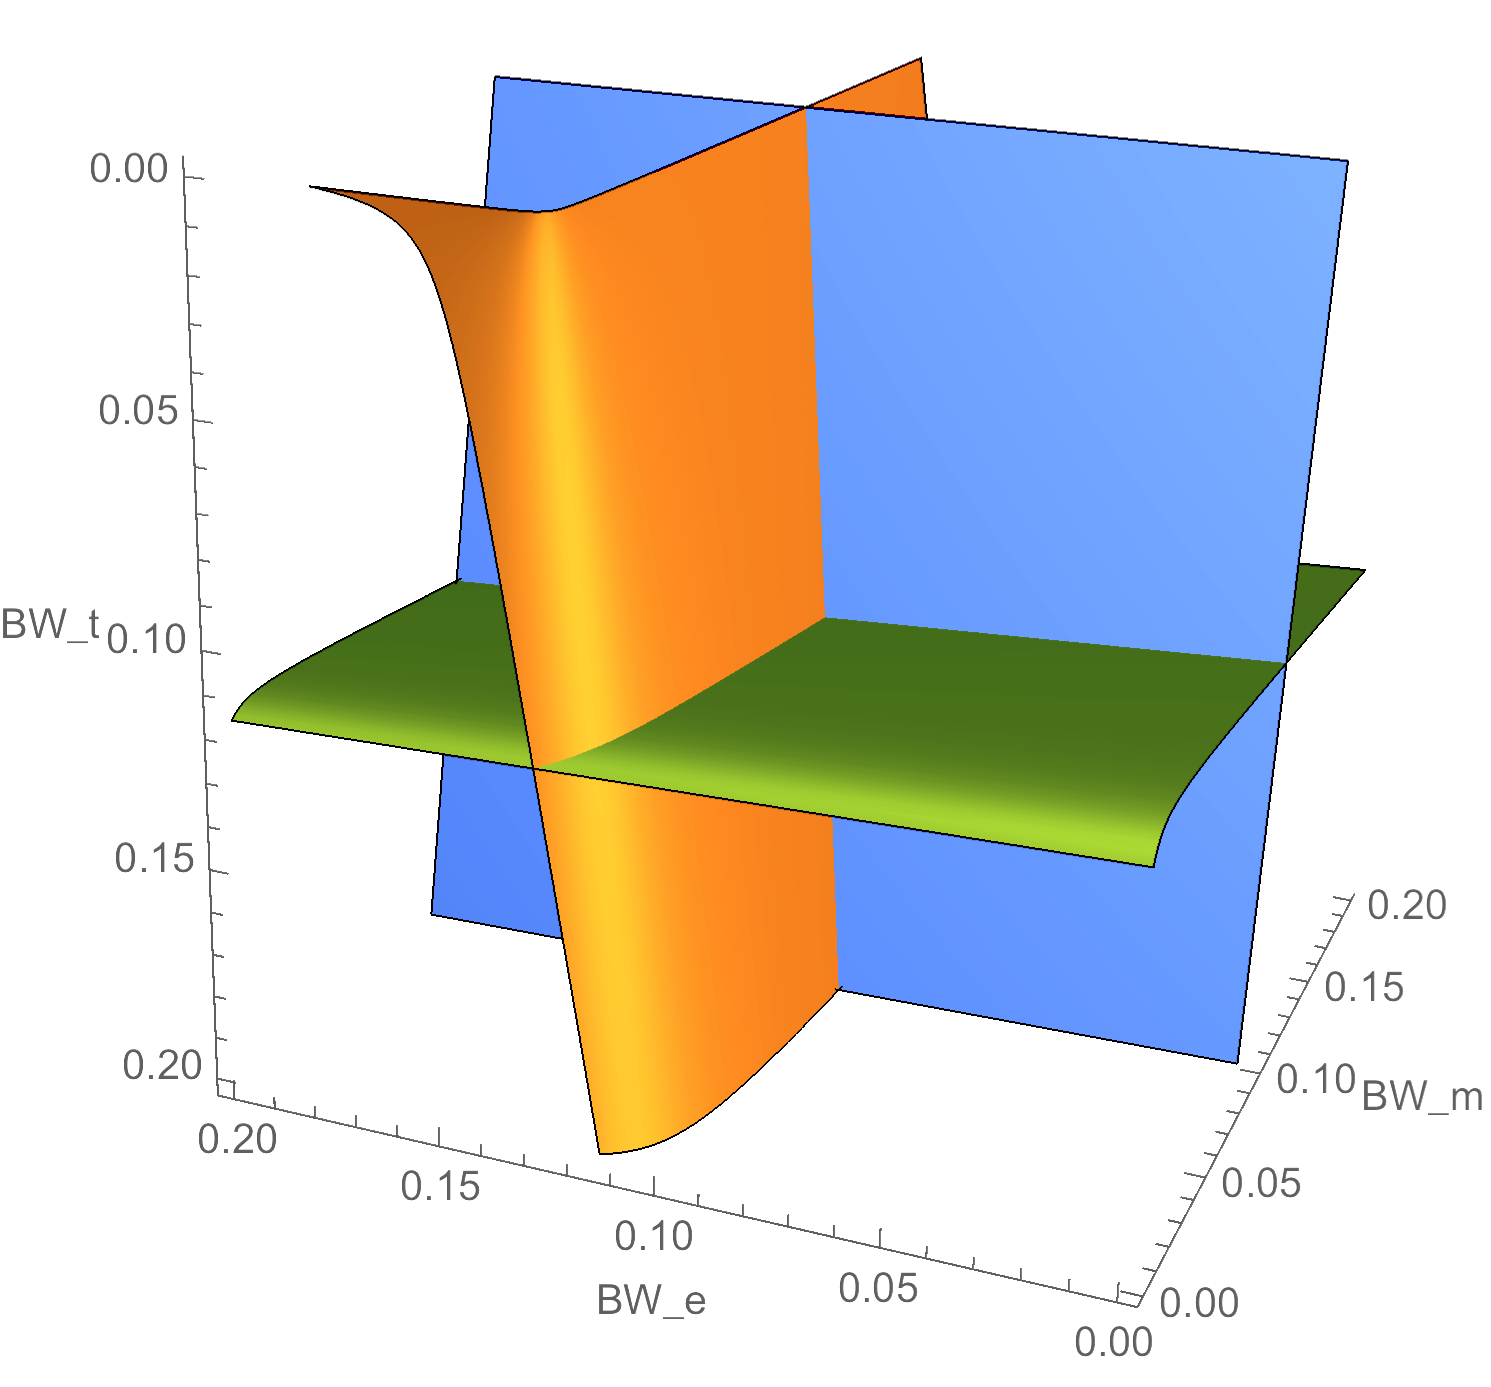
\includegraphics[width=7cm]{chapters/Analysis/sectionStatisticalAnalysis/figures/visual.png}
    
    %--------------------------
    \caption{Visualization of Eq \ref{quadEqB} in the
    \(\{\beta_{e},\beta_{\mu},\beta_{\tau}\}\) parameter space. Each
    equation in Eq \ref{quadEqB} is a hyperbolic plane, while their
    intersection is the solution Eq \ref{quadEqB}. Mathematically, there
    are 8 possible solutions. However, only one solution is physical,
    located with \(\beta \in (0,1) \). }
    \label{visualize}
\end{figure}

% This approach analytically obtains the coefficient $c_{ij}$ in 
% Eq \ref{quadEqB} from efficiency matrix \textbf{E} and measured 
% normalized yields $\{X_{e},X_{\mu},X_{\tau}\}$. Then it numerically
% solves the branching fractions $\{\beta_{e},\beta_{\mu},\beta_{\tau}\}$,
% using a modification of the Powell hybrid method as implemented in MINPACK-Scipy. 

\begin{equation} 
    \left [
    \begin{tabular}{c}
	    $\beta_{e}$ \\
	    $\beta_{\mu}$ \\
	    $\beta_{\tau}$
    \end{tabular}
    \right ]
    = Solution
    \left [
    \begin{tabular}{c}
	    $Q_e    (\beta_e,\beta_\mu,\beta_\tau) = 0$ \\
	    $Q_\mu  (\beta_e,\beta_\mu,\beta_\tau) = 0$ \\
	    $Q_\tau (\beta_e,\beta_\mu,\beta_\tau) = 0$
    \end{tabular}
\right ]
\end{equation}

\FloatBarrier

%%%%%%%%%%%%%%%%%%%%%%%%%%%%%%%%%%%%%%%%
% 3. Test of Parameters Extraction
%%%%%%%%%%%%%%%%%%%%%%%%%%%%%%%%%%%%%%%%
\subsection{Test of Parameters Extraction}


A test of parameter extraction is performed using
signal MC samples, in which $\beta=10.80\%$ is assumed. The test
takes $N_{mc,sg}$ as input instead of data yields with background 
subtracted $n=N_{data} - N_{mc,bg}$, 
so as to check whether the extracted branching fractions agree with 
the assumption in signal simulation.

we generate 2000 toys, each of which variates the yield $n=N_{sg}$ by $\delta_n=\sqrt{N_{sg}}$.
The distribution of $\{\beta_{e},\beta_{\mu},\beta_{\tau}\}$ extracted from toys are shown in
figure~\ref{test_toy}. The centers of distributions are consistent with
the assumed branching fraction in the MC generator, while widths of distributions are 
consistent with uncertainty calculated by error propagation.


\begin{figure}[ht]
    \centering
    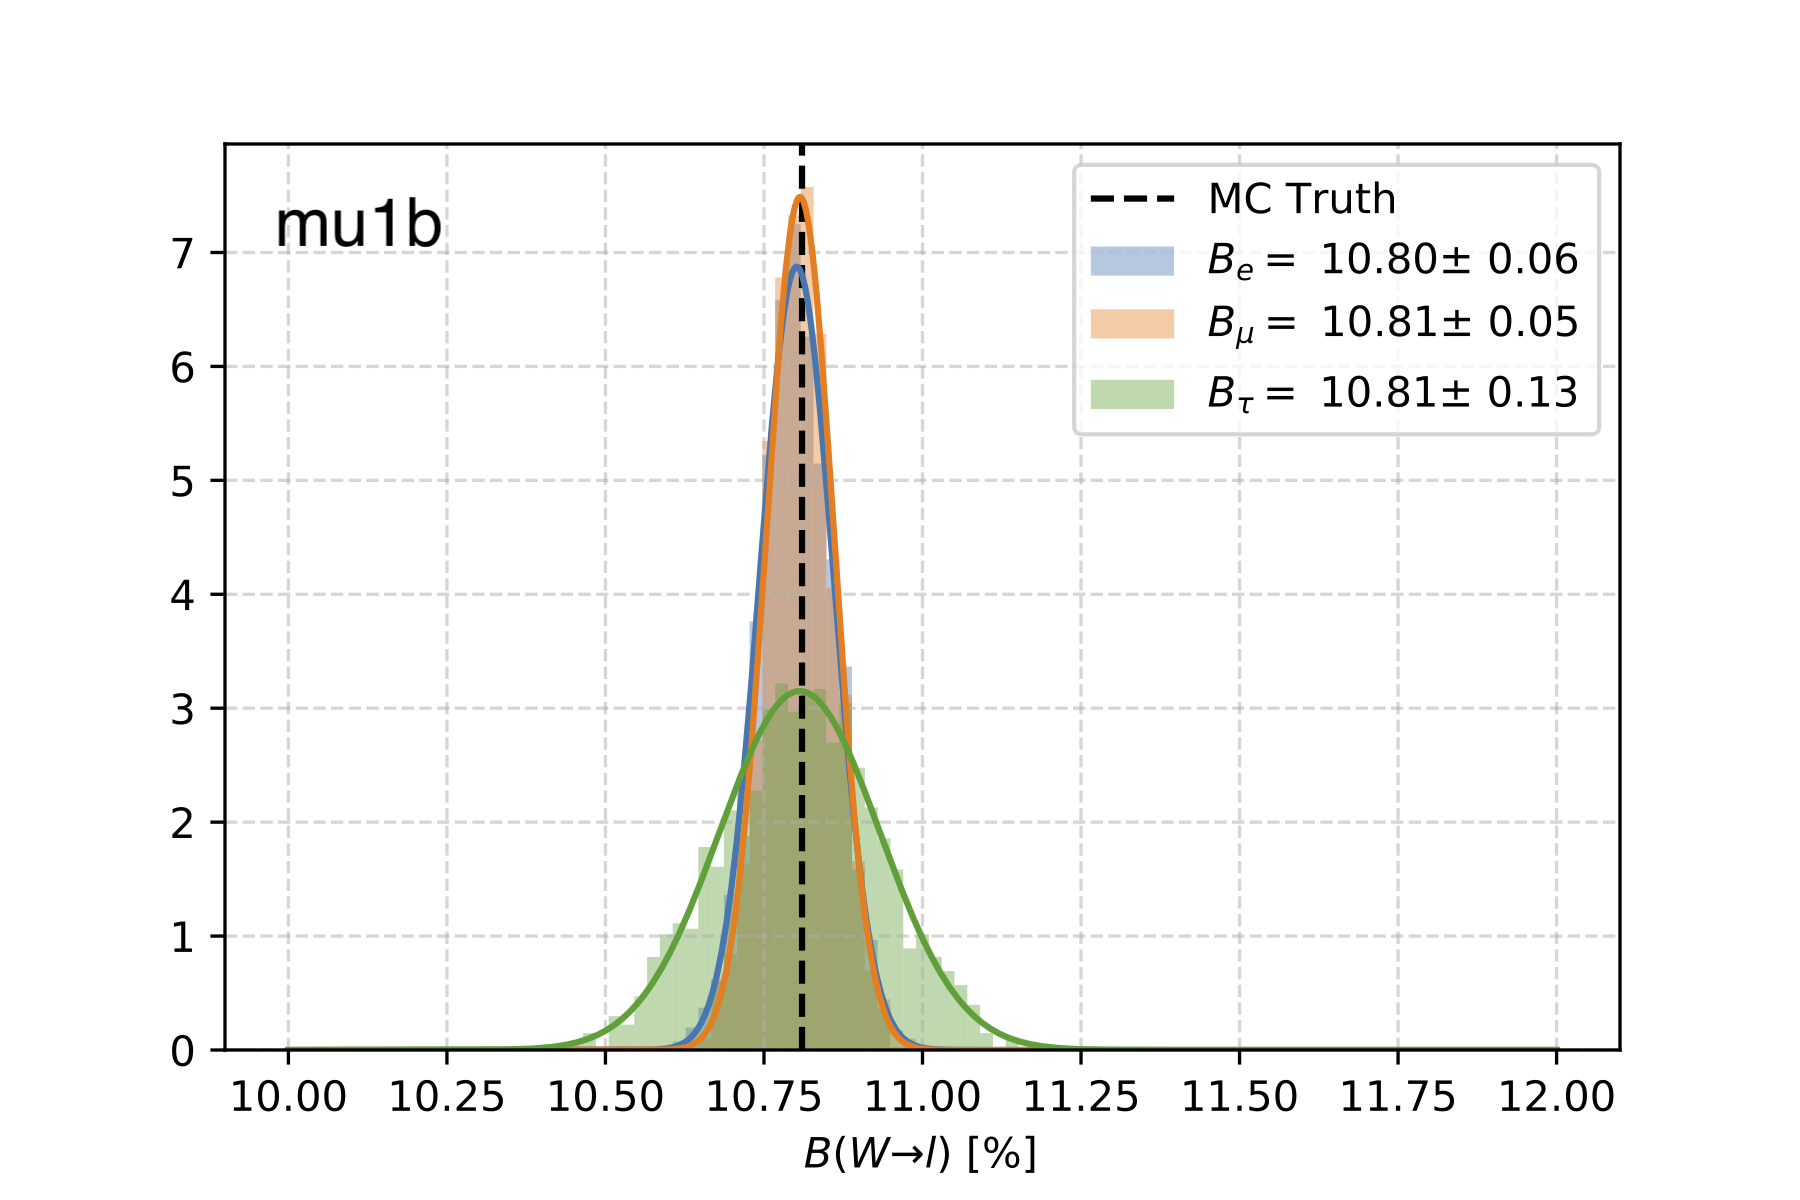
\includegraphics[width=7cm]{chapters/Analysis/sectionStatisticalAnalysis/figures/test_mu1b.png}
    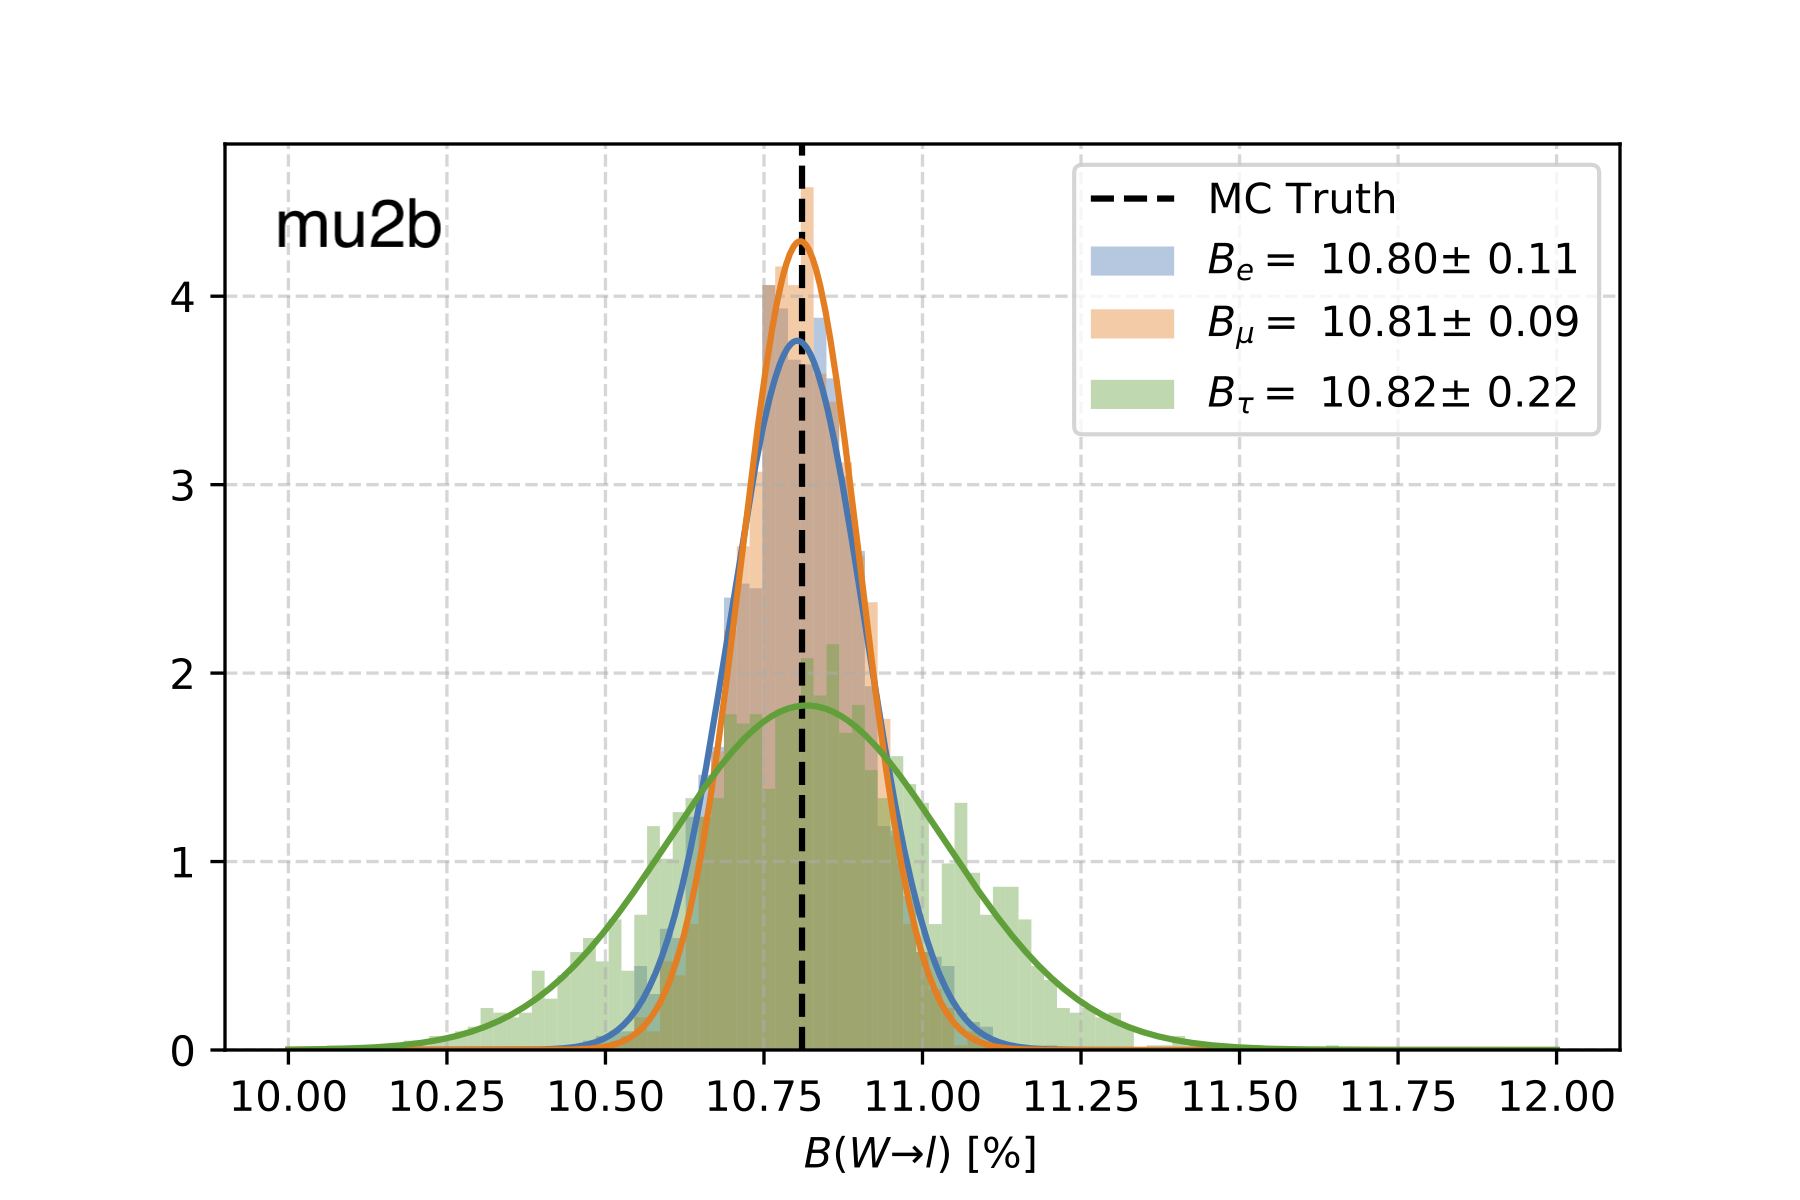
\includegraphics[width=7cm]{chapters/Analysis/sectionStatisticalAnalysis/figures/test_mu2b.png}
    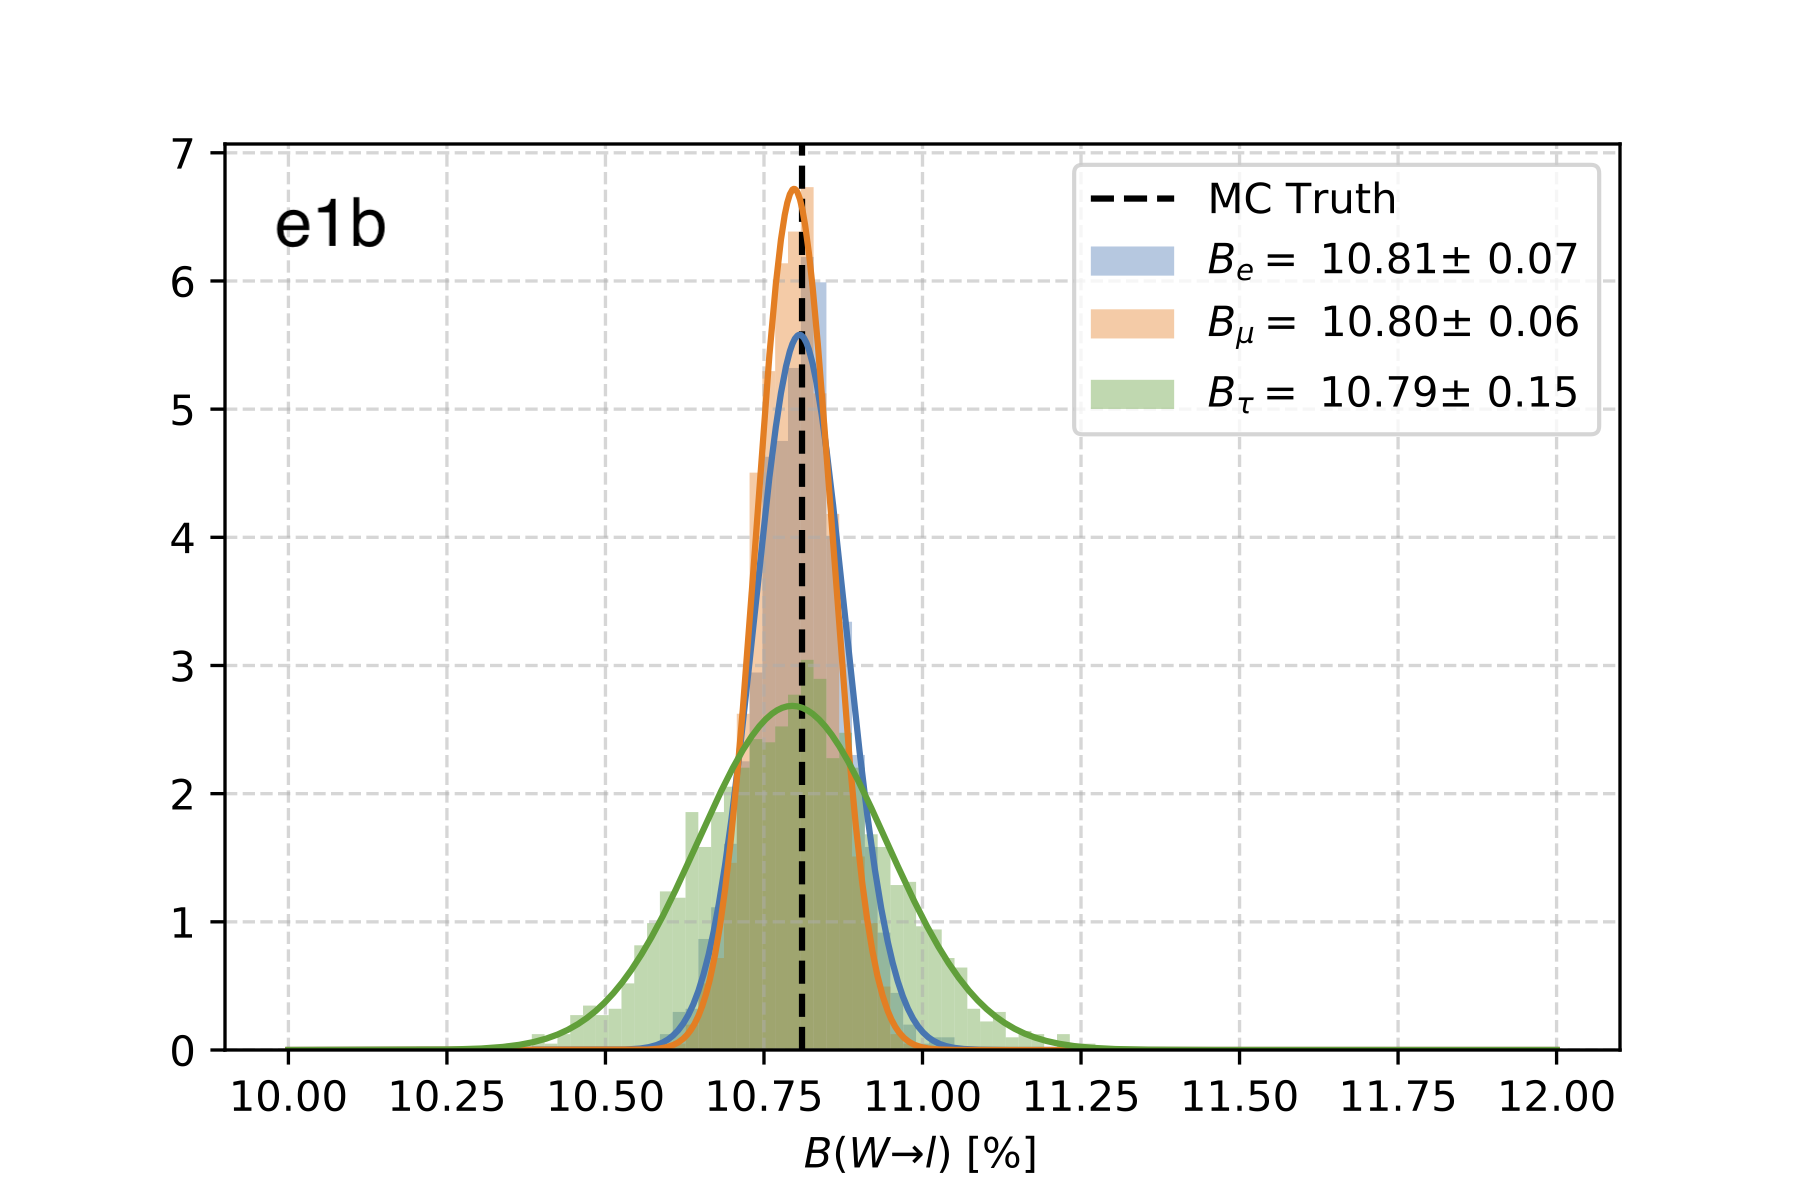
\includegraphics[width=7cm]{chapters/Analysis/sectionStatisticalAnalysis/figures/test_e1b.png}
    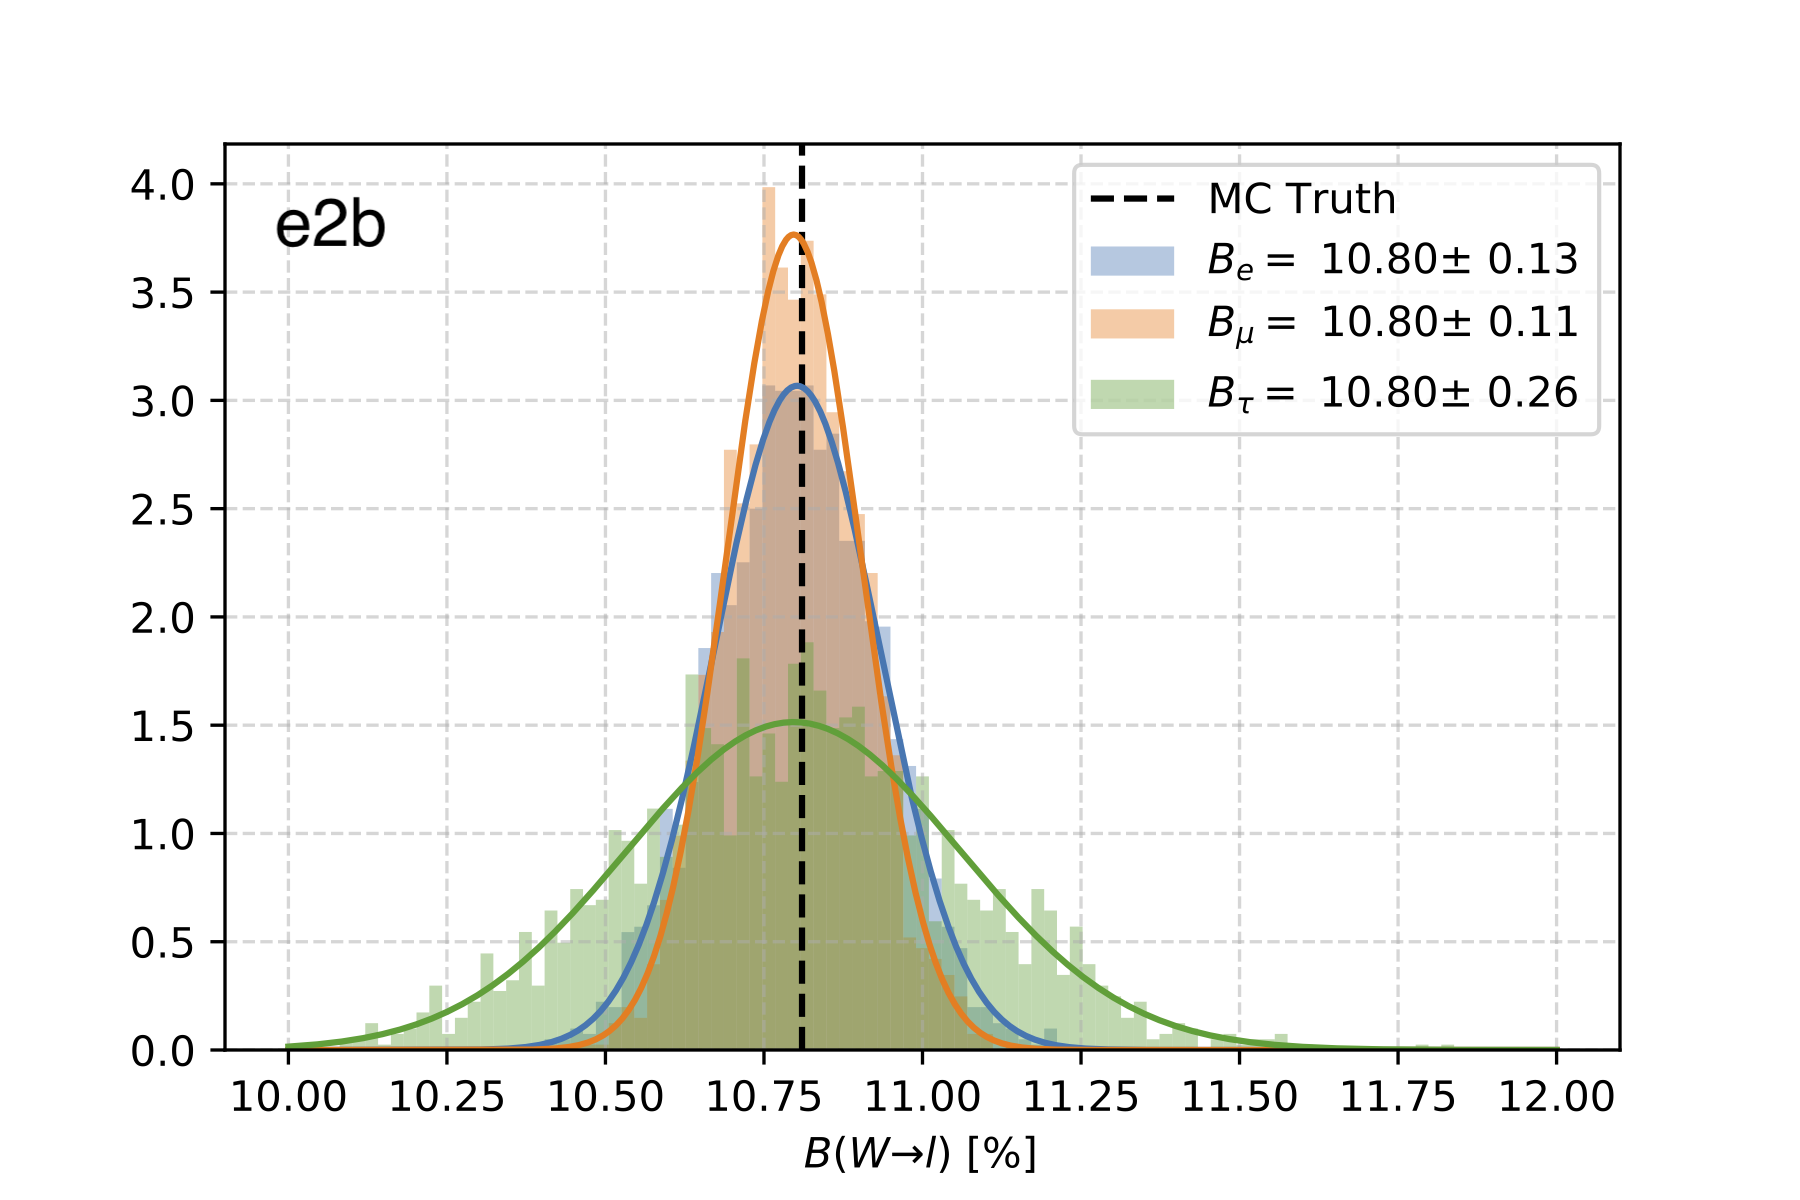
\includegraphics[width=7cm]{chapters/Analysis/sectionStatisticalAnalysis/figures/test_e2b.png}
    
    %--------------------------
    \caption{ Distribution of 2000 toys. }
    \label{test_toy}
\end{figure}

\begin{quote}
    
    After establishing parameter extraction, we perform a closure test using 
    signal MC samples. As is described above, the input of parameter extraction 
    is data yields with background subtracted $n=N_{data} - N_{mc,bg}$. 
    But here for testing purpose, we replace $n=N_{data} - N_{mc,bg}$ with $N_{mc,sg}$ as the input,
    as is given in Eqn \ref{eqn:testinput}.
    The pass of the test is that parameter extraction 
    gives back branching fraction assumed in the MC generator, which is $10.80\%$.
    
    
    \begin{equation}
    	n=N_{mc,sg}\pm \sqrt{N_{mc,sg}}
    	\label{eqn:testinput}
    \end{equation}
    
    where $N_{mc,sg}$ comes from tt and tW MC sample normalized to luminosity. 
    It is uncertainty is assumed as a Gaussian error with width $\sqrt{N_{sg}}$, 
    so as to estimate the expected statistical uncertainty of data.
    The extracted branching fraction is listed in Table \ref{test_ana}.

\end{quote}



\begin{table}[ht]
    \centering
	\begin{tabular}{l|ccc}
    \hline
          	 & $B_e$             &   $B_\mu$       	 & 	  $B_\tau$   	 \\
    MC Assumption  & 10.80 		 &  10.80 		 	 & 	  10.80     	 \\
    \hline
  	$\mu-1b$ &   10.802$\pm$0.058  &   10.807$\pm$0.053  &    10.808$\pm$0.127 \\
  	$\mu-2b$ &   10.802$\pm$0.103  &   10.807$\pm$0.092  &    10.808$\pm$0.216 \\
  	$e-1b$   &   10.804$\pm$0.073  &   10.797$\pm$0.059  &    10.794$\pm$0.152 \\
  	$e-2b$   &   10.805$\pm$0.130  &   10.797$\pm$0.104  &    10.794$\pm$0.263 \\
    \hline
	\end{tabular}
	
	%--------------------------
    \caption{Branching fraction extracted from signal MC. The 
    uncertainty is calculated by error propagation. The small 
    deviation from MC assumption is resulted by the difference 
    value of $Br(\tau \to e)$ and $Br(\tau \to \mu)$ in MC and in 
    extractor. The extractor uses 0.1773,0.1731 respectively, while 
    the MC assumption of tau decay needs to be found in generator 
    cards. 
    }
    \label{test_ana}
\end{table}

\FloatBarrier

% In addition, to test the error propagation, we generate 2000 toy experiments, 
% each of which variates the yield $n=N_{sg}$ by $\sqrt{N_{sg}}$.
% The width of distribution of toys is consistent with uncertainty 
% from error propagation list in the Table \ref{test_ana}.
% Also as expected, the center of distribution of toys is consistent with
% the assumed branching fraction in the MC generator.






% Finally, the branching fractions obtained in all four categories are combined:

% \begin{equation}
% 	\beta_i = \frac{ \sum_{cat} \beta_i^{cat} / \sigma^2_{\beta_i^{cat}}}{\sum_{cat} 1 / \sigma^2_{\beta_i^{cat}}} ,
%     \qquad
%     \sigma^2_{\beta_i} = \frac{1}{\sum_{cat} 1 / \sigma^2_{\beta_i^{cat}} }
% \end{equation}

% where $i = e,\mu,\tau$ and categories are single electron or muon trigger with 1 or 2 b-jets, $cat \in \{\mu \text{-} 1b,\mu \text{-} 2b,e \text{-} 1b,e \text{-} 2b \}$

